\documentclass[11pt]{article}
\usepackage{xeCJK}
\usepackage[a4paper, margin=1.4in]{geometry}
\usepackage{fancyhdr}
\usepackage{amsmath}
\usepackage{amssymb}
\usepackage{graphicx}
\usepackage[most]{tcolorbox}
\usepackage{framed} 
\usepackage{tikz}
\usepackage{hyperref}

\linespread{1.25}
\setlength\parindent{0pt}

\title{%
  \LARGE
  \textbf{COMP90086 Computer Vision \\
  \large Week 3
  \\
  Light, Shadow and Edges}}
\author{ Lecture Notes summarized by Neo }
\date{Semester 2 2021}

\pagestyle{fancy}
\fancyhf{}
\rhead{COMP90086 Computer Vision}
\lhead{Lecture Notes}
\rfoot{Page \thepage}

\begin{document}

\maketitle

\section{Image Formation}

\begin{figure}[hbt!]
    \centering
    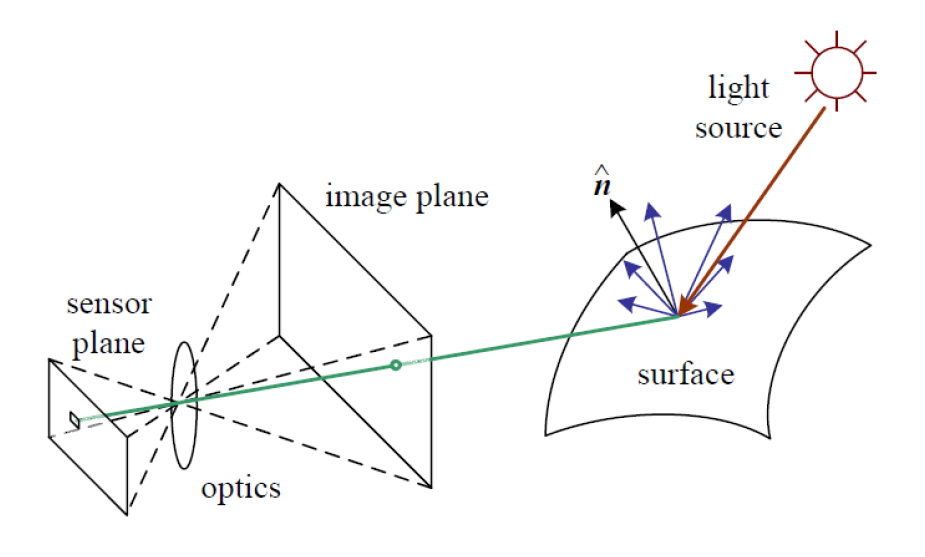
\includegraphics[width=0.8\textwidth]{image_formation.png}
    \caption{Image formation model}
\end{figure}
\subsection{Diffuse (Lambertian) reflectance 漫反射(漫射)}
表面一般为粗糙的。
\begin{Large}
    $$I_D(x)=I_LRN(x)\cdot L$$
\end{Large}
where
\begin{itemize}
    \item $I_D$ is the Intensity of reflected light
    \item $I_L$ is the light source intensity (在CV处理中常忽略)
    \item $R$ is the surface colour (reflectance)
    \item $N(x)$ is the surface normal vector
    \item $L$ is the vector to light source
\end{itemize}

\begin{framed}
    \begin{center}
        The goal is to recover \textbf{both} the surface colour and the normal vector given the reflected light.
    \end{center}
\end{framed}

\section{Colour}
\subsection{Visible Light}
\begin{figure}[hbt!]
    \centering
    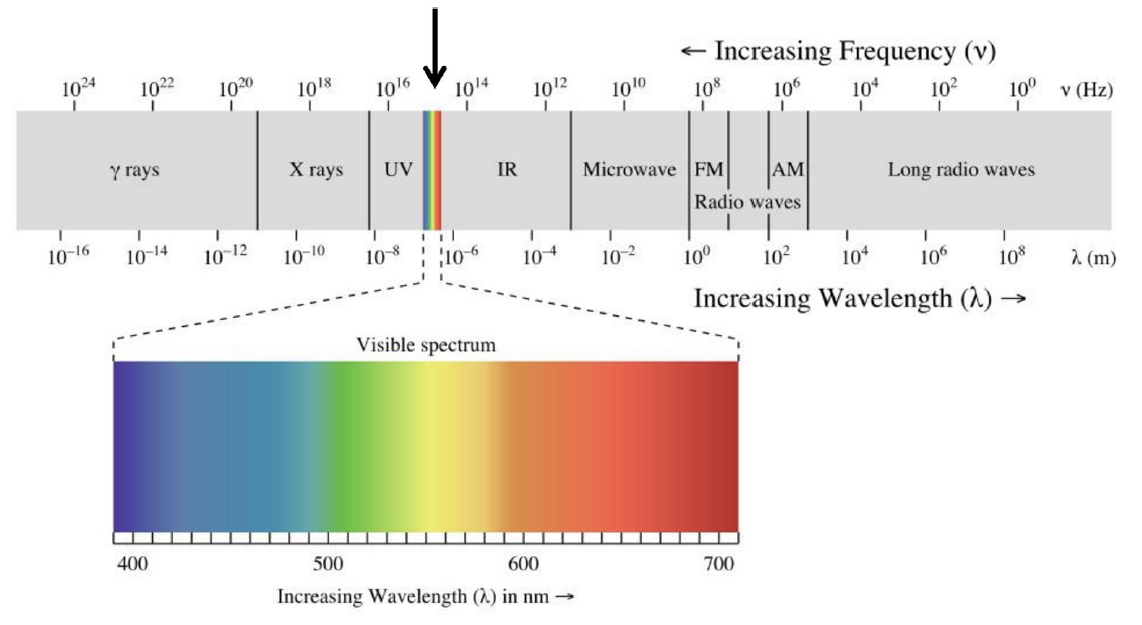
\includegraphics[width=\textwidth]{visible_light.png}
    \caption{Visible light spectrum}
\end{figure}
频率与波长成反比,频率越大颜色越冷,越小越暖。

\subsection{Perceived Colour}
大部分人类的视网膜上有\textbf{三种}感知颜色的感光细胞,叫做视锥细胞,分别对不同波长的光线敏感,称为 L/M/S 型细胞。三种视锥细胞最敏感的波长分别是橙红色(长波,Long),绿色(中波,Medium),蓝色(短波,Short)。这三种视锥细胞的归一化感光曲线如下图所示。\footnote{https://zhuanlan.zhihu.com/p/24214731}

世界上所有颜色,在人类的眼里看到,最后传送到大脑里的信号,就只有这三种视锥细胞的电信号而已。根据这三种电信号的强弱,大脑解读成了不同的颜色。
\begin{figure}[hbt!]
    \centering
    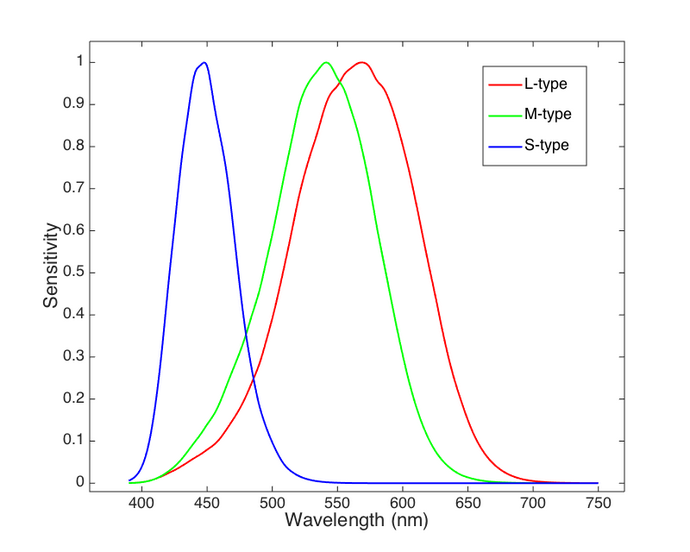
\includegraphics[width=0.8\textwidth]{perceived.png}
    \caption{Light response spectra of human eyes}
\end{figure}

\begin{framed}
    \begin{center}
        世界上每一种颜色都是这三种电信号的组合,并且同样的颜色会有无数种三种电信号组合的方式。
    \end{center}
\end{framed}

\subsubsection*{Sensor Response (Perceived value of light)}
\begin{itemize}
    \item $I_R=\int_{700}^{400}I(\lambda)S_R(\lambda)\, \partial \lambda$
    \item $I_G=\int_{700}^{400}I(\lambda)S_G(\lambda)\, \partial \lambda$
    \item $I_B=\int_{700}^{400}I(\lambda)S_B(\lambda)\, \partial \lambda$
\end{itemize}

下图为一个例子:上面的图代表Spectrum,产出相同的颜色。(误差不好控制)
\begin{figure}[hbt!]
    \centering
    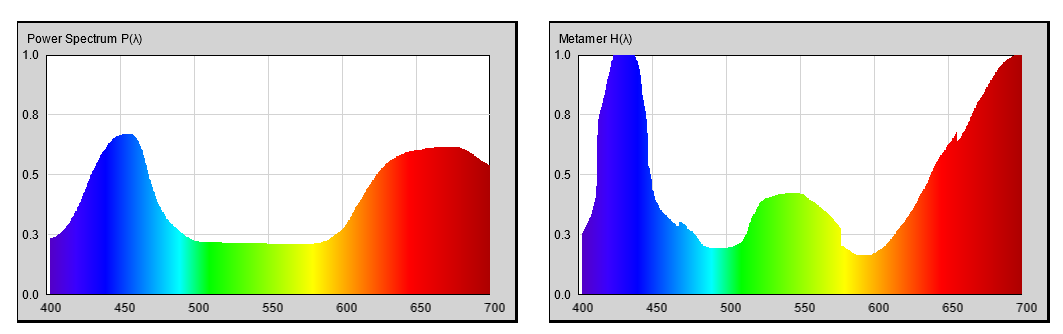
\includegraphics[width=\textwidth]{diff1.png}
\end{figure}
\begin{figure}[hbt!]
    \centering
    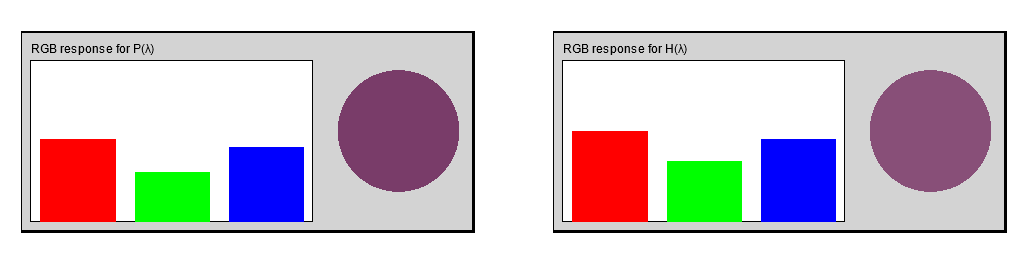
\includegraphics[width=\textwidth]{diff2.png}
    \caption{Different spectrum, same colour}
\end{figure}

\newpage
\subsection{Colour Representation}
常见的颜色表示方式:
\begin{itemize}
    \item RGB(注意有不同版本的RGB定义)
    \item HSL/HSV (Hue色相 Saturation饱和度 Lightness亮度/Value明度)
    \item CIE 1931 XYZ(Colourmatch RGB)
    \item LAB (luminance, a*=red/green, b*=blue/yellow)
\end{itemize}
\begin{figure}[hbt!]
    \centering
    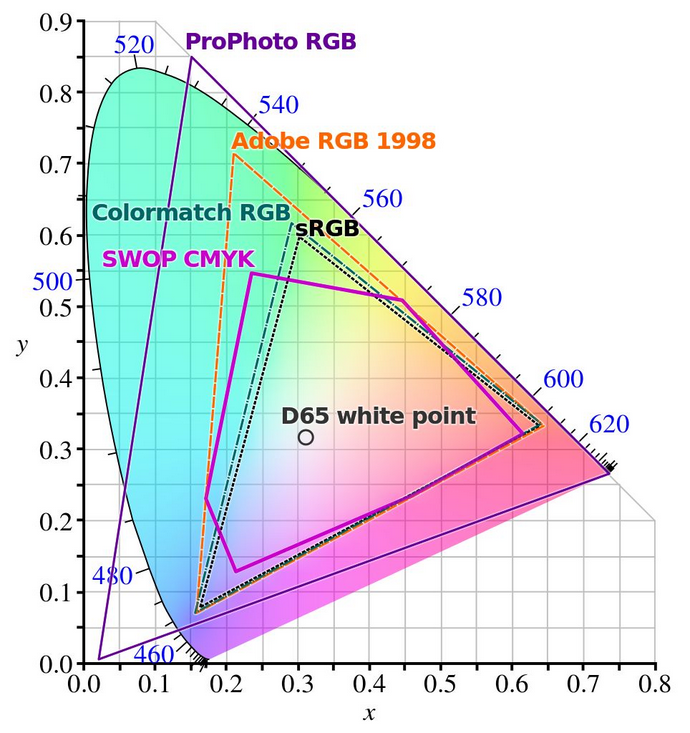
\includegraphics[width=0.88\textwidth]{colour_space.png}
    \caption{Colour spaces}
\end{figure}


\subsection{Colour Transforms}
由于 CIE XYZ 空间是一个很方便的线性空间,与具体设备无关,因此常用来做各种颜色空间转换的中间媒介。设想某个颜色的光,经过色匹配函数的计算,得到了三个 XYZ 的值,如果直接将这三个值作为 RGB 颜色显示到屏幕上,显然是不对的。我们必须把 XYZ 的值转换到屏幕的 RGB 空间中的值。反之同理。\\(built-in functions in OpenCV)
$$\left[\begin{matrix}X\\Y\\Z\end{matrix}\right]=M\ \left[\begin{matrix}R\\G\\B\end{matrix}\right]$$

\newpage
色谱图的构造实现(超纲):\url{https://zhuanlan.zhihu.com/p/24281841}
\subsection{Colour Swap}
不要在RGB Space中直接交换颜色因为\textbf{亮度}与颜色在RGB里有联系,直接交换会导致亮度不统一。\textbf{转化成LAB Space会有更好的结果},因为亮度与颜色分离。


\section{Shading and Surfaces}
\subsection{Recovering Surface Normal}
Assume no changes in surface colour..
$$I_D(x)=N(x)\cdot L=\cos \theta_x$$

Can only recover angle between surface normal and light source, but not normal
\\
However, can add additional assumptions:
\begin{itemize}
    \item Normals along boundary of object are known
    \item Neighbouring normal are similar
\end{itemize}
\begin{framed}
    \begin{center}
        已知的条件不足以推断出Surface Normal Vector,只能计算出Normal和光源的夹角。计算Normal通常需要大量的Assumption,因为人眼做了大部分Assumption所以可以推断出物体的“Surface”。
    \end{center}
\end{framed}
\subsection{Recovering Surface Reflectance}
\begin{figure}[hbt!]
    \centering
    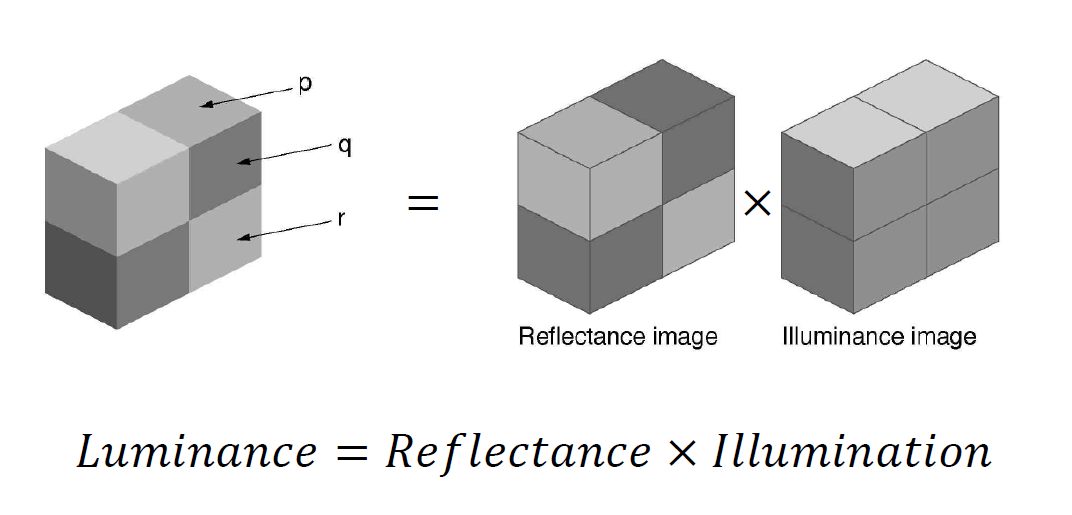
\includegraphics[width=\textwidth]{lum.png}
\end{figure}
\subsubsection{Simple Approach}
Simple approach: assume illumination variation
produces low spatial frequency changes in image,
remove illumination in frequency domain.
\begin{enumerate}
    \item $L=R\times I$
    \item $\ln (L)=\ln (R) + \ln (I)$
    \item $FT(\ln (L))=FT(\ln (R)) + FT(\ln (I))$
    \item Apply a high pass filter 𝑔in the frequency domain
    \item $Image=e^{FT^{-1}(g\times FT(\ln (L)))}$
\end{enumerate}

\subsubsection{Problems}
\begin{itemize}
    \item Some reflectance edges are smooth
    \item Some lighting edges are not smooth (textures, corners)
\end{itemize}
More sophisticated approaches (e.g., based on
partial differential equations) can give better
results but have similar problems.
\begin{framed}
    \begin{center}
        Lighting usually isn't uniform and most surfaces aren't matte/Lambertian.
    \end{center}
\end{framed}

\section{Edge Detection}
Edges are caused by a variety of factors:
\begin{itemize}
    \item Surface normal discontinuity(表面角度变化)
    \item Depth discontinuity (change in depth but not in colour)
    \item Surface colour discontinuity
    \item Illumination discontinuity(投射阴影,常忽略)
\end{itemize}



\begin{framed}
    \begin{center}
        Edges are points in the image with a high change in intensity = high change in gradient.
    \end{center}
\end{framed}



\subsection{Canny Algorithm}
The Canny edge detector is an edge detection operator that uses a multi-stage algorithm to detect a wide range of edges in images. It was developed by John F. Canny in 1986. Canny also produced a computational theory of edge detection explaining why the technique works.
\begin{itemize}
    \item Noice reduction
    \item Gradient calculation
    \item Non-maximum Suppression
    \item Double threshold
    \item Edge Tracking by Hysteresis
\end{itemize}

\begin{figure}[hbt!]
    \centering
    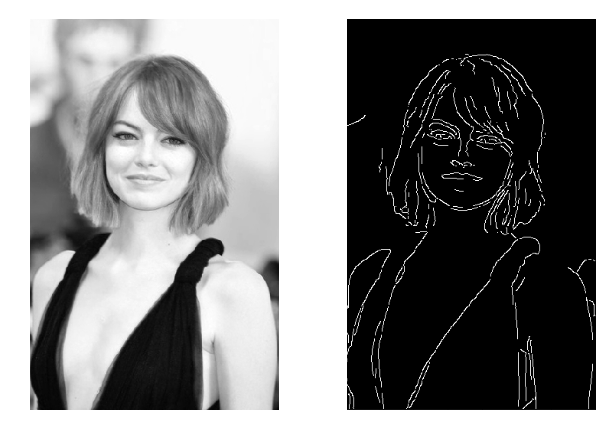
\includegraphics[width=0.8\textwidth]{canny.png}
    \caption{Original image on the left and final image on the right}
\end{figure}

\subsubsection{Noise Reduction}
Since the mathematics involved behind the scene are mainly based on derivatives
(cf. Step 2: Gradient calculation),
edge detection results are highly sensitive to image noise.
One way to get rid of the noise on the image,
is by applying Gaussian blur to smooth it.
To do so, image convolution technique is applied with a
Gaussian Kernel (3x3, 5x5, 7x7 etc…).
The kernel size depends on the expected blurring effect.
Basically, the smallest the kernel, the less visible is the blur.
\begin{figure}[hbt!]
    \centering
    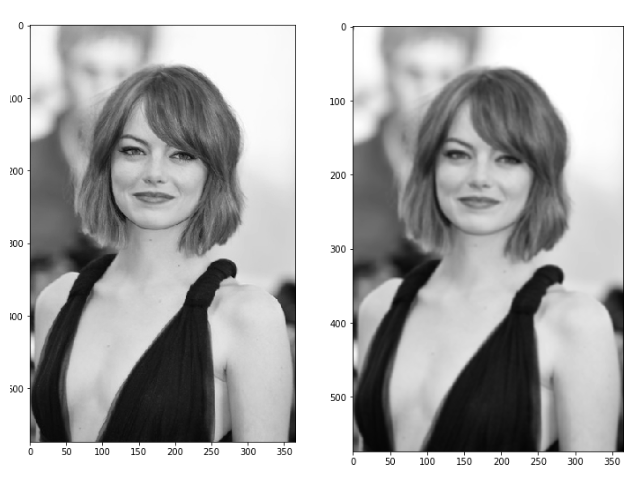
\includegraphics[width=0.7\textwidth]{canny1.png}
    \caption{Processed with noice reduction}
\end{figure}


\subsubsection{Gradient Calculation}
The Gradient calculation step detects the edge intensity and direction by calculating the gradient of the image using edge detection operators.
\begin{framed}
    \begin{center}
        Edges correspond to a change of pixels’ intensity. To detect it, the easiest way is to apply filters that highlight this intensity change in both directions: horizontal ($x$) and vertical ($y$).
    \end{center}
\end{framed}

When the image is smoothed, the derivatives $I_x$ and $I_y$ w.r.t. $x$ and $y$ are calculated. It can be implemented by convolving I with Sobel kernels $K_x$ and $K_y$, respectively:

$$K_x=\left[\begin{matrix}-1&0&1\\-2&0&2\\-1&0&1\end{matrix}\right],\ K_y=\left[\begin{matrix}1&2&1\\0&0&0\\-1&-2&-1\end{matrix}\right]$$

Then, the magnitude $G$ and the slope $\theta$ of the gradient are calculated as follow:
$$\left|G\right|=\sqrt{I_x^2+I_y^2},$$
$$\theta\left(x,\ y\right)=\arctan\left(\frac{I_y}{I_x}\right)$$

\begin{figure}[hbt!]
    \centering
    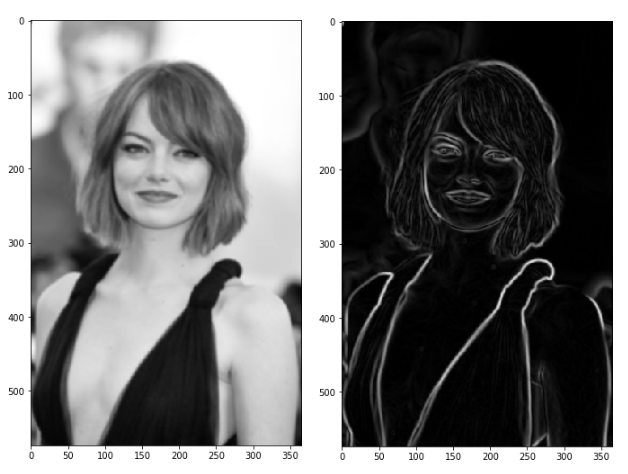
\includegraphics[width=0.7\textwidth]{canny2.png}
    \caption{Processed with gradient calculation}
\end{figure}


The result is almost the expected one, but we can see that some of the edges are thick and others are thin. Non-Max Suppression step will help us mitigate the thick ones.

Moreover, the gradient intensity level is between 0 and 255 which is not uniform. The edges on the final result should have the same intensity (i-e. white pixel = 255).


\subsubsection{Non-Maximum Suppression}
Ideally, the final image should have thin edges. Thus, we must perform non-maximum suppression to thin out the edges.

The principle is simple: maximum suppression: If nearby pixels claim to be
part of the same edge, only keep the one with
maximum gradient.

如果原图像有渐变过来的边界算法可能会计算出很粗的边界(很多个连在一起),为了保证边界粗细统一我们使用Non-Maximum Suppression。

\begin{itemize}
    \item Bin edges by orientation
    \item For each edge pixel:
          \begin{enumerate}
              \item Check the two neighbour pixels orthogonal to this edge pixel,
              \item If either neighbour has same edge orientation AND higher magnitude, this pixel is not an edge.
          \end{enumerate}
\end{itemize}

\begin{figure}[hbt!]
    \centering
    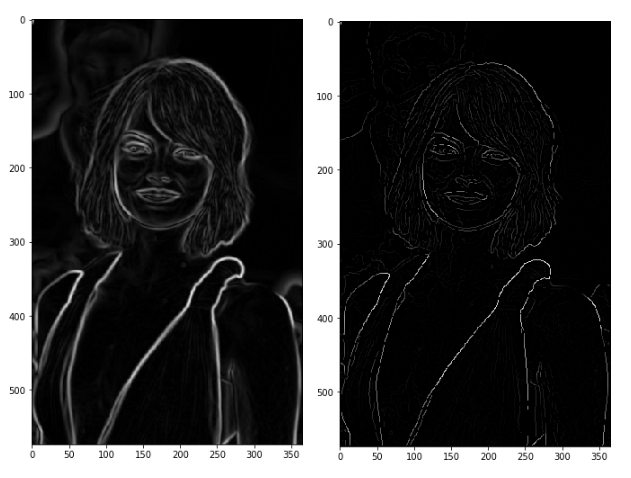
\includegraphics[width=0.7\textwidth]{canny3.png}
    \caption{Processed with non-maximum suppression}
\end{figure}

The result is the same image with thinner edges. We can however still notice some variation regarding the edges’ intensity: some pixels seem to be brighter than others, and we will try to cover this shortcoming with the two final steps.


\subsubsection{Thresholding with hysteresis (combined the last two steps)}
\begin{itemize}
    \item Two thresholds $T_1, T_2$ with $T_1 > T_2$
    \item Strong edges: magnitude $> T_1$
    \item Weak edges: $T_1 >$ magnitude $> T_2$
    \item For each weak edge:
          \begin{enumerate}
              \item Check the 8 pixel neighbourhood around this pixel
              \item If any neighbour is a strong edge, relabel the weak edge
                    pixel as a strong edge
          \end{enumerate}
    \item Final edge map = strong edges
\end{itemize}

\begin{figure}[hbt!]
    \centering
    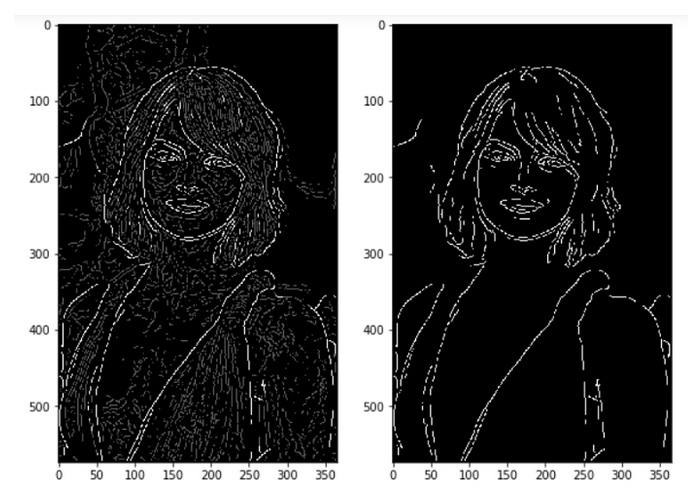
\includegraphics[width=0.8\textwidth]{canny4.png}
    \caption{Processed with thresholding with hysteresis}
\end{figure}


\section{Image Recognition}
\subsection{Compression}
\begin{itemize}
    \item Edge = discontinuity
    \item Efficient way to represent images: only represent points
          where the signal changes (e.g., Elder \& Zucker, 1996)
\end{itemize}

\subsection{Invariance}
\begin{itemize}
    \item Edge based features are invariant or tolerant to many
          irrelevant image changes
    \item Invariant to $X$ = response/representation does not
          vary with $X$, is insensitive to changes in $X$
    \item Tolerant to $X$ = response is mostly insensitive to $X$
\end{itemize}

\subsection{Image Recognition}
More on next weeks...

\subsection{Hough transform}
......



\end{document}
